%\begin{frame}
%    \centering
%    \Large{Part I:}\\
%    \ \\
%    \ \\
%    \centering
%    \Large{Adaptive order polynomial algorithm in a\\
%            multiwavelet representation scheme}
%\end{frame}


%\begin{frame}
%\frametitle{Multiwavelets}
%\begin{columns}
%\begin{column}[b]{0.55\linewidth}
%\begin{itemize}
%    \item   \textbf{Scaling functions} are polynomials or order $\leq k$\\
%	    on the unit interval
%    \item   \textbf{Dilation and translation} to refinement scale $n$
%	    \begin{equation}
%		\nonumber
%		\phi_l^n(x) = 2^{n/2}\phi(2^nx-l)
%	    \end{equation}
%    \item   At scale $n$ there are $2^n$ subintervals
%    \item   The length of each subinterval is $2^{-n}$
%    \item   \textbf{Scaling projection} at scale $N$
%	    \begin{equation}
%		\nonumber
%		f(x) \approx f^N(x) = \sum_l s_l^N \phi_l^N(x)
%	    \end{equation}
%	    \ \\
%	    \ \\
%    \item   For a $k$-order basis in $d$ dimensions there are\\
%	    $\left(2(k+1)\right)^{nd}$ basis functions at scale $n$\\
%\end{itemize}
%\centering
%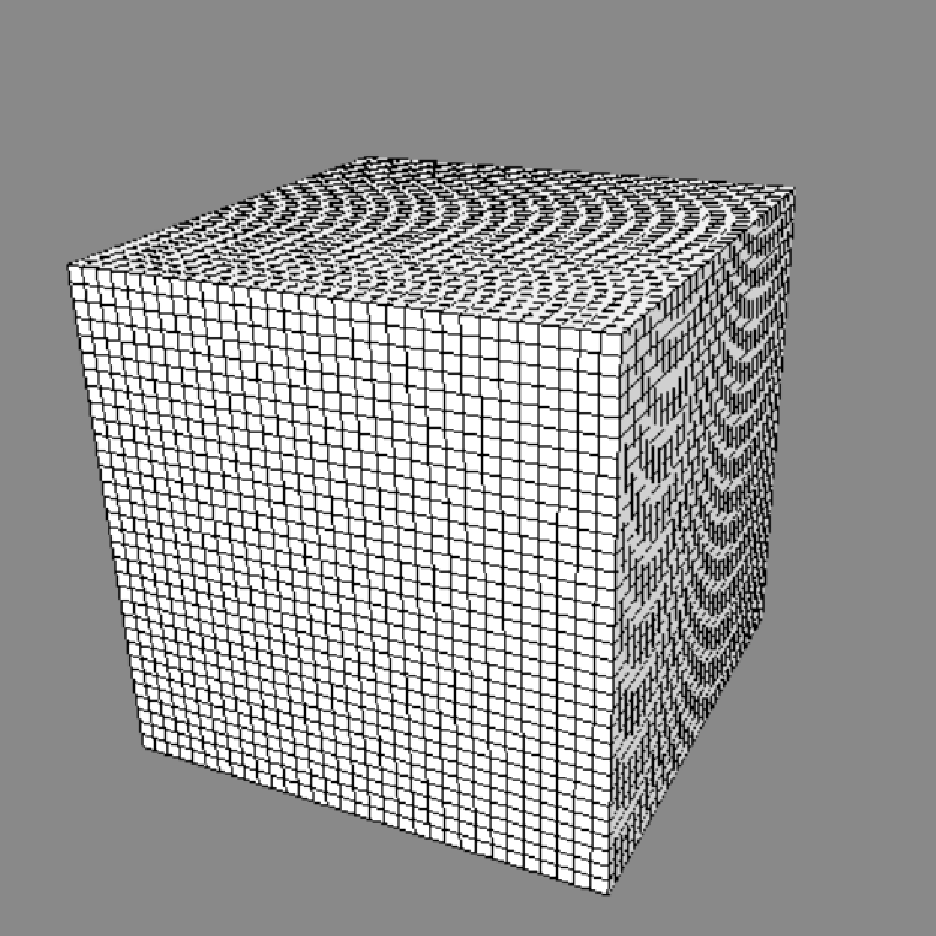
\includegraphics[scale=0.2]{figures/unifgrid.pdf}
%\end{column}
%
%\begin{column}[b]{0.45\linewidth}
%\centering
%\includegraphics[scale=0.3, clip, viewport=150 450 450 750]
%    {figures/scaling.pdf}\\
%\includegraphics[scale=0.3, clip, viewport=100 400 500 800]
%    {figures/refinement.pdf}
%\end{column}
%
%\end{columns}
%\end{frame}

\begin{frame}
\frametitle{Multiwavelets}
\centering
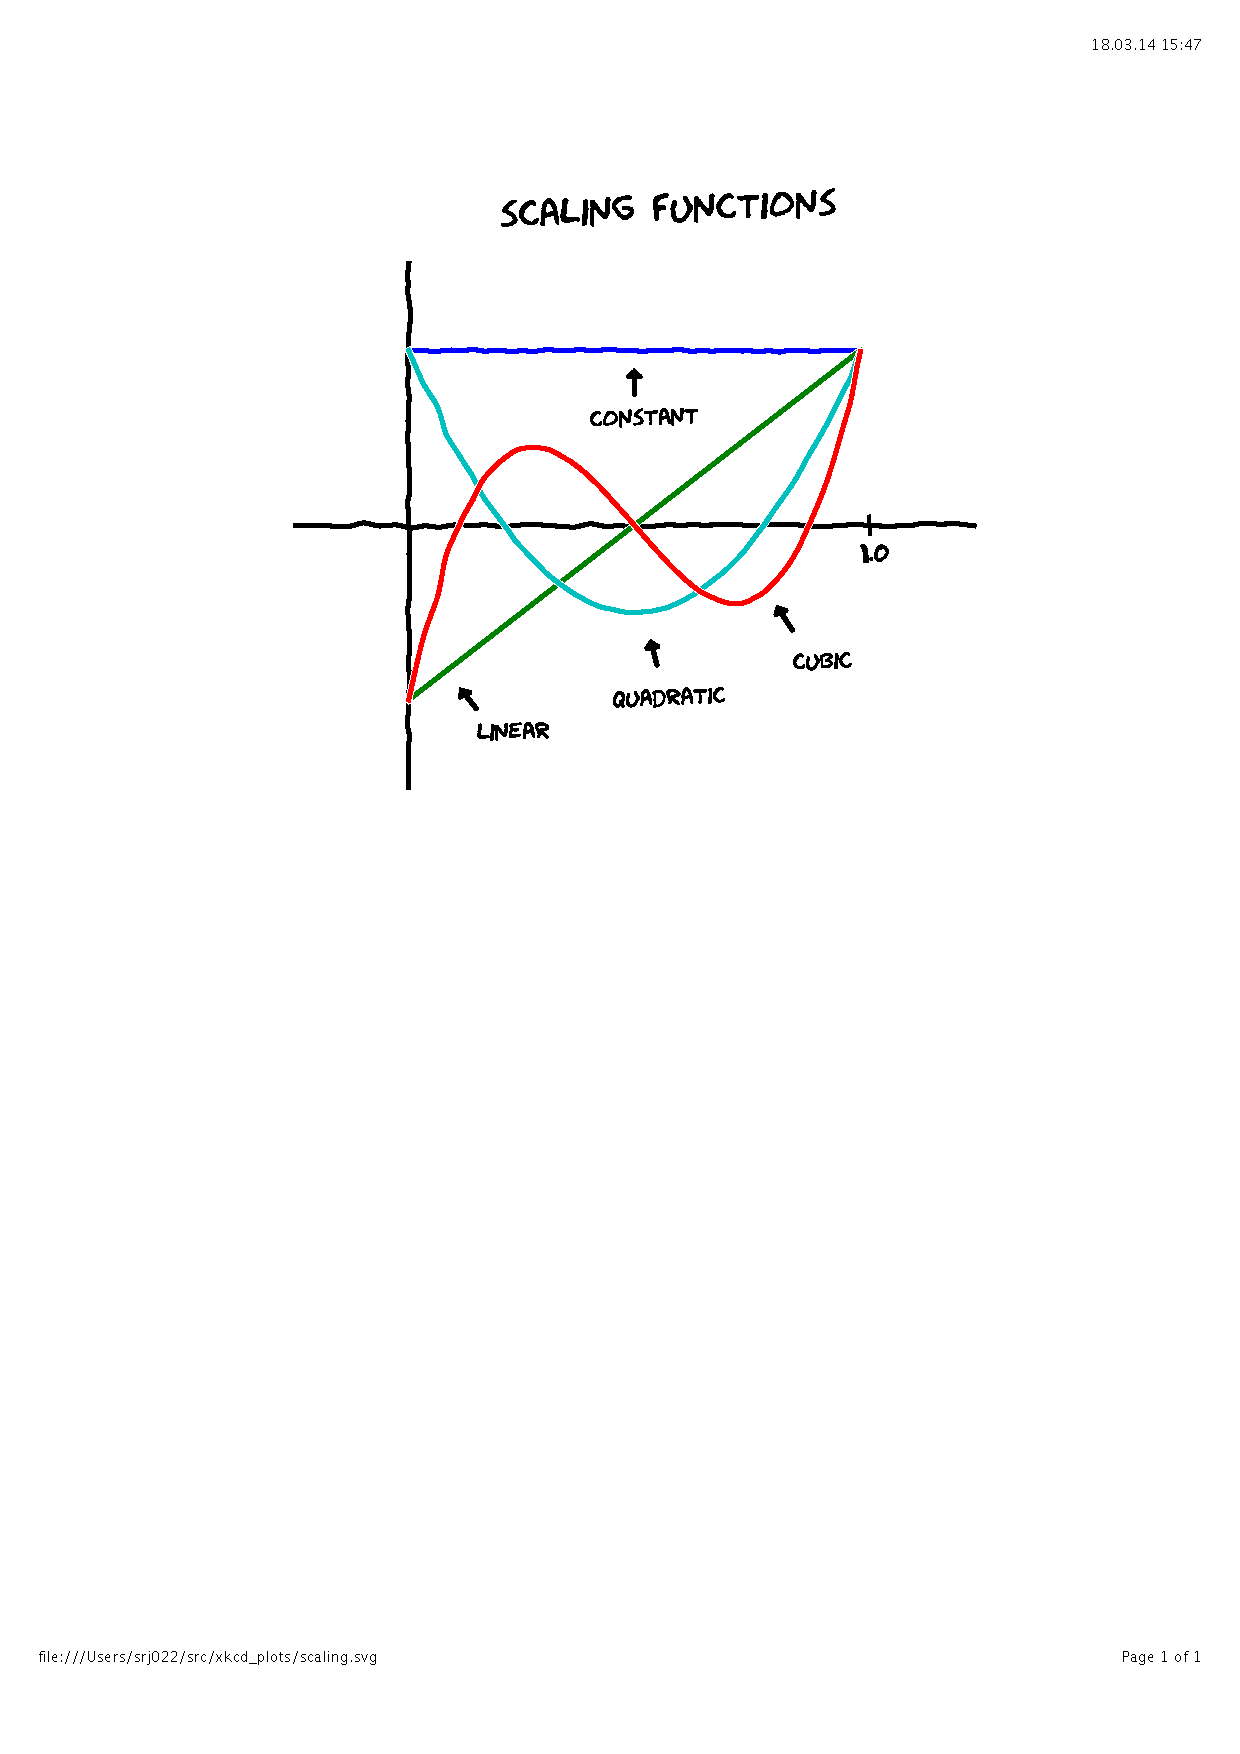
\includegraphics[scale=0.5, clip, viewport=150 450 450 750]{figures/scaling.pdf}
\end{frame}

%\begin{frame}
%\frametitle{Multiwavelets}
%\centering
%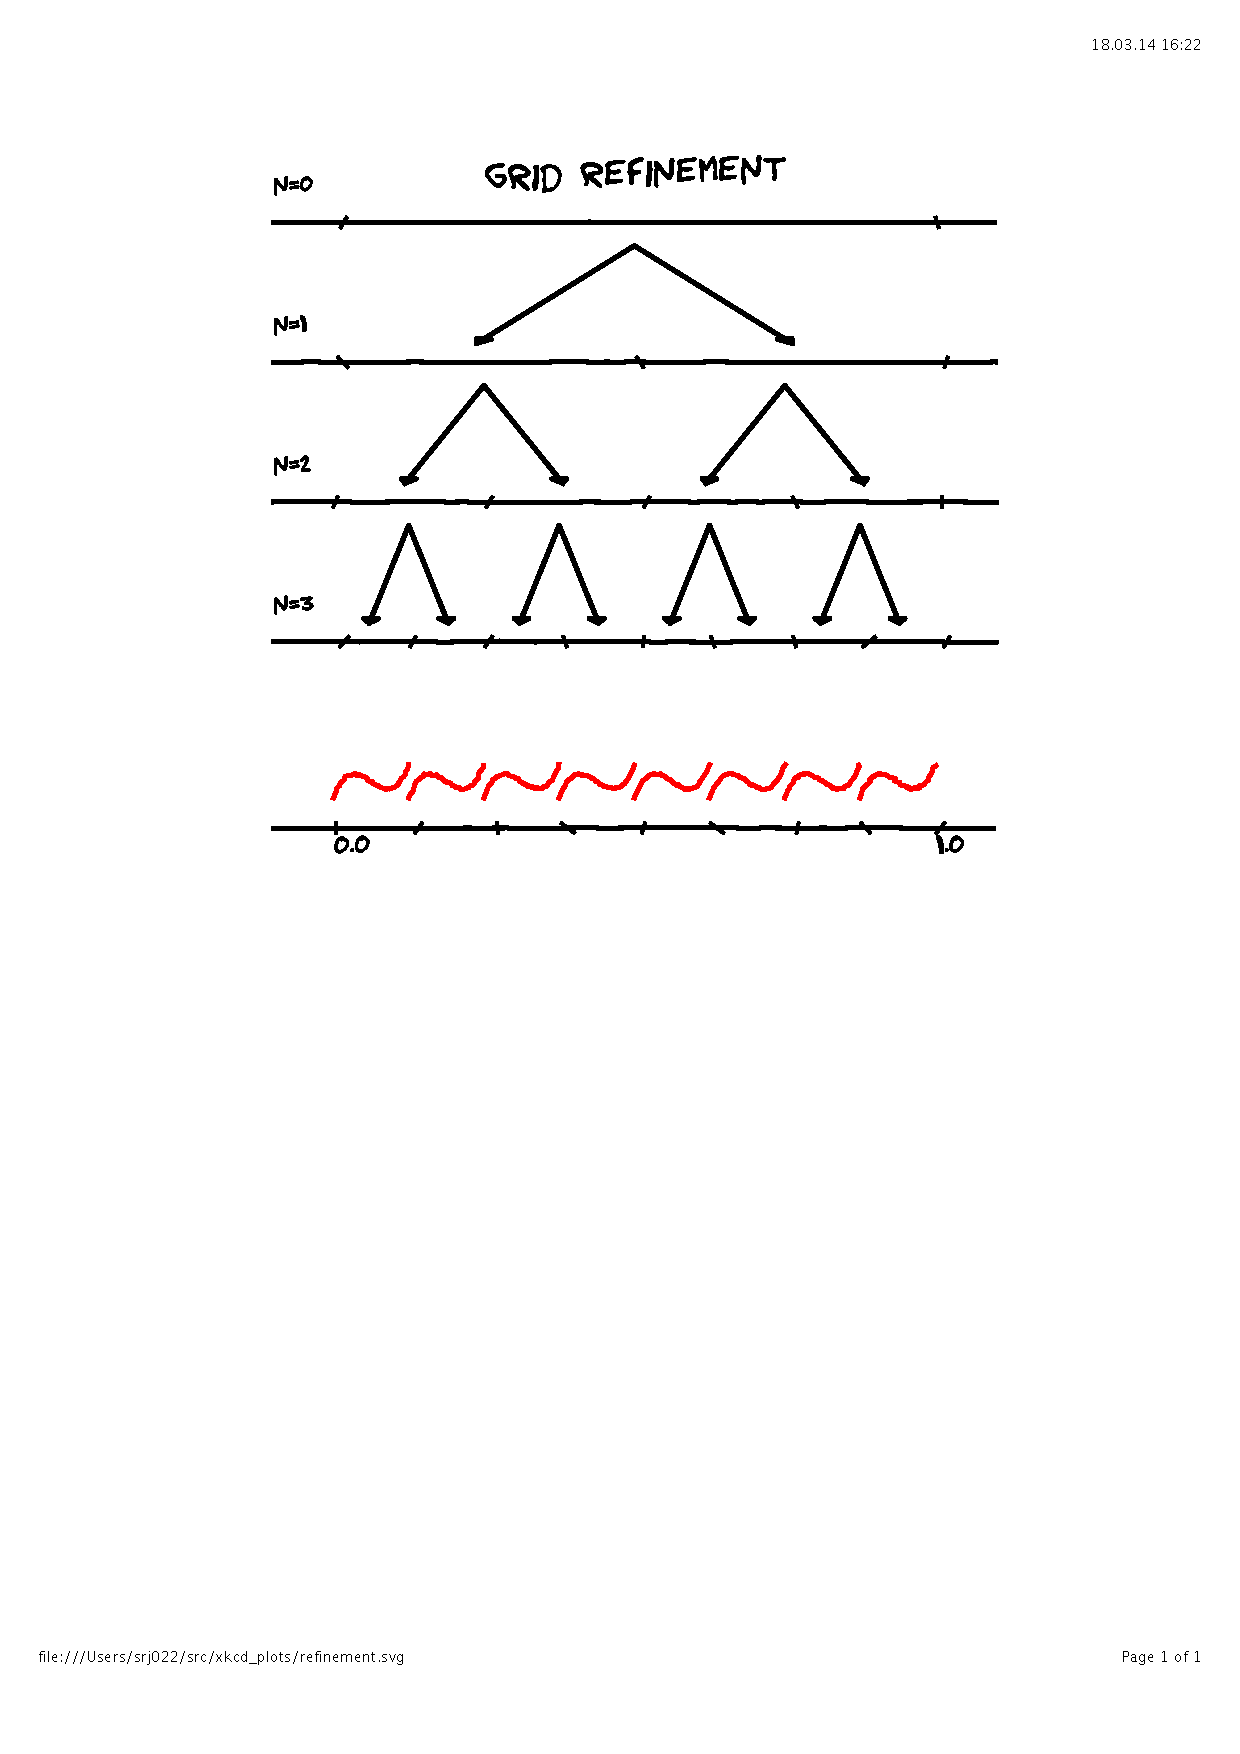
\includegraphics[scale=0.5, clip, viewport=100 400 500 800]{figures/refinement.pdf}
%\end{frame}

%\begin{frame}
%\frametitle{Multiwavelets}
%\centering
%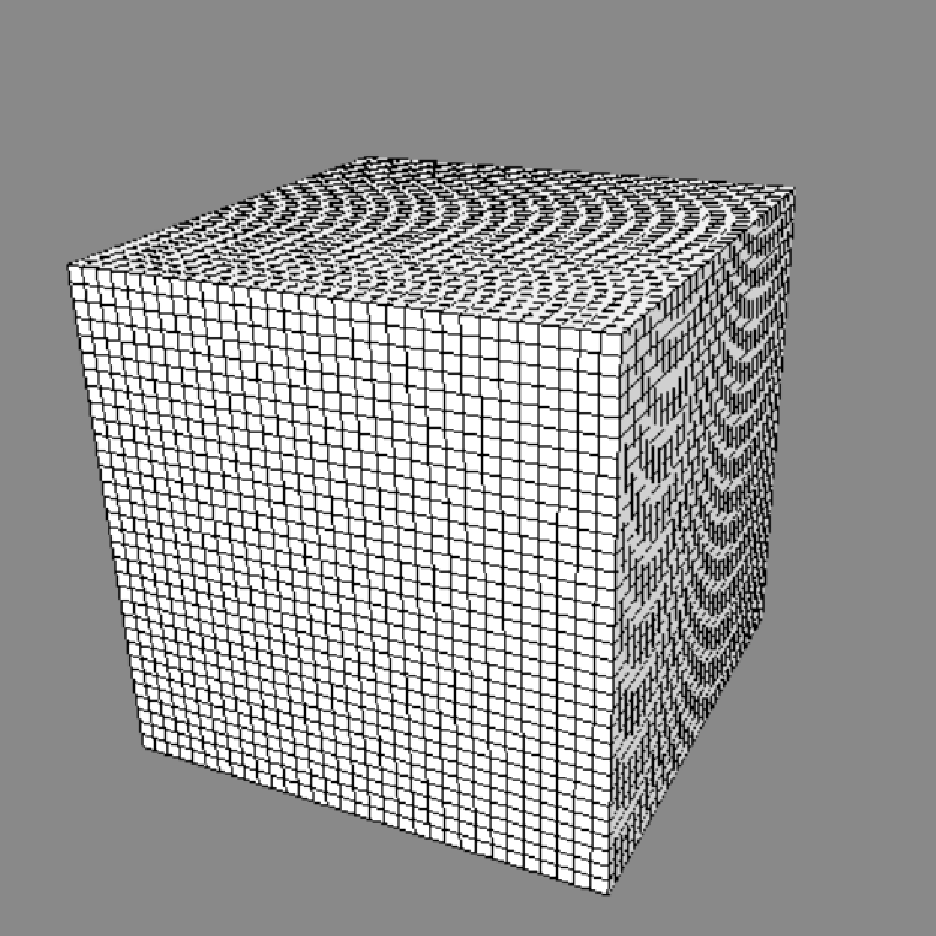
\includegraphics[scale=0.35]{figures/unifgrid.pdf}
%\end{frame}

\begin{frame}
\frametitle{Multiwavelets}
\centering
\only<1>{\ \ \ 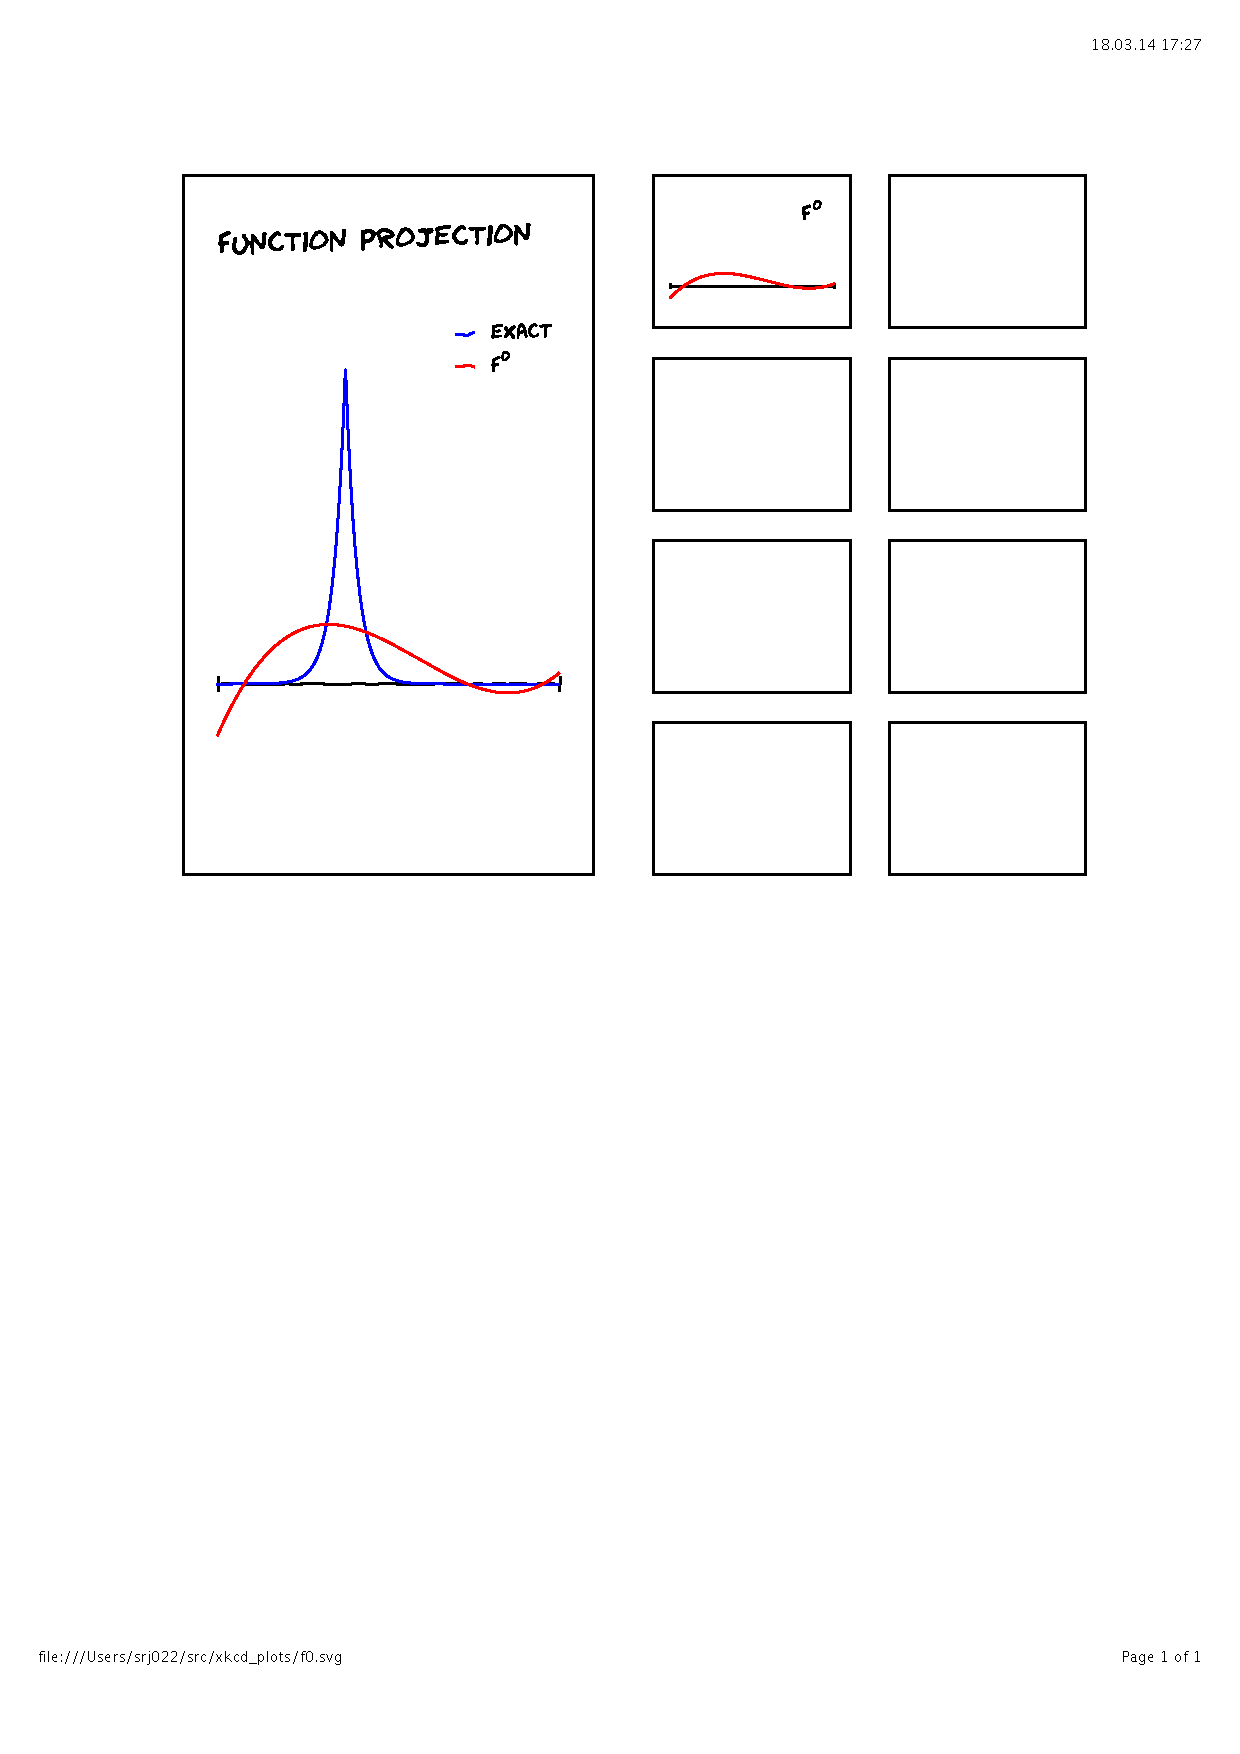
\includegraphics[clip, viewport=50 100 600 800, scale=0.5]
    {figures/f0.pdf}}
\only<2>{\ \ 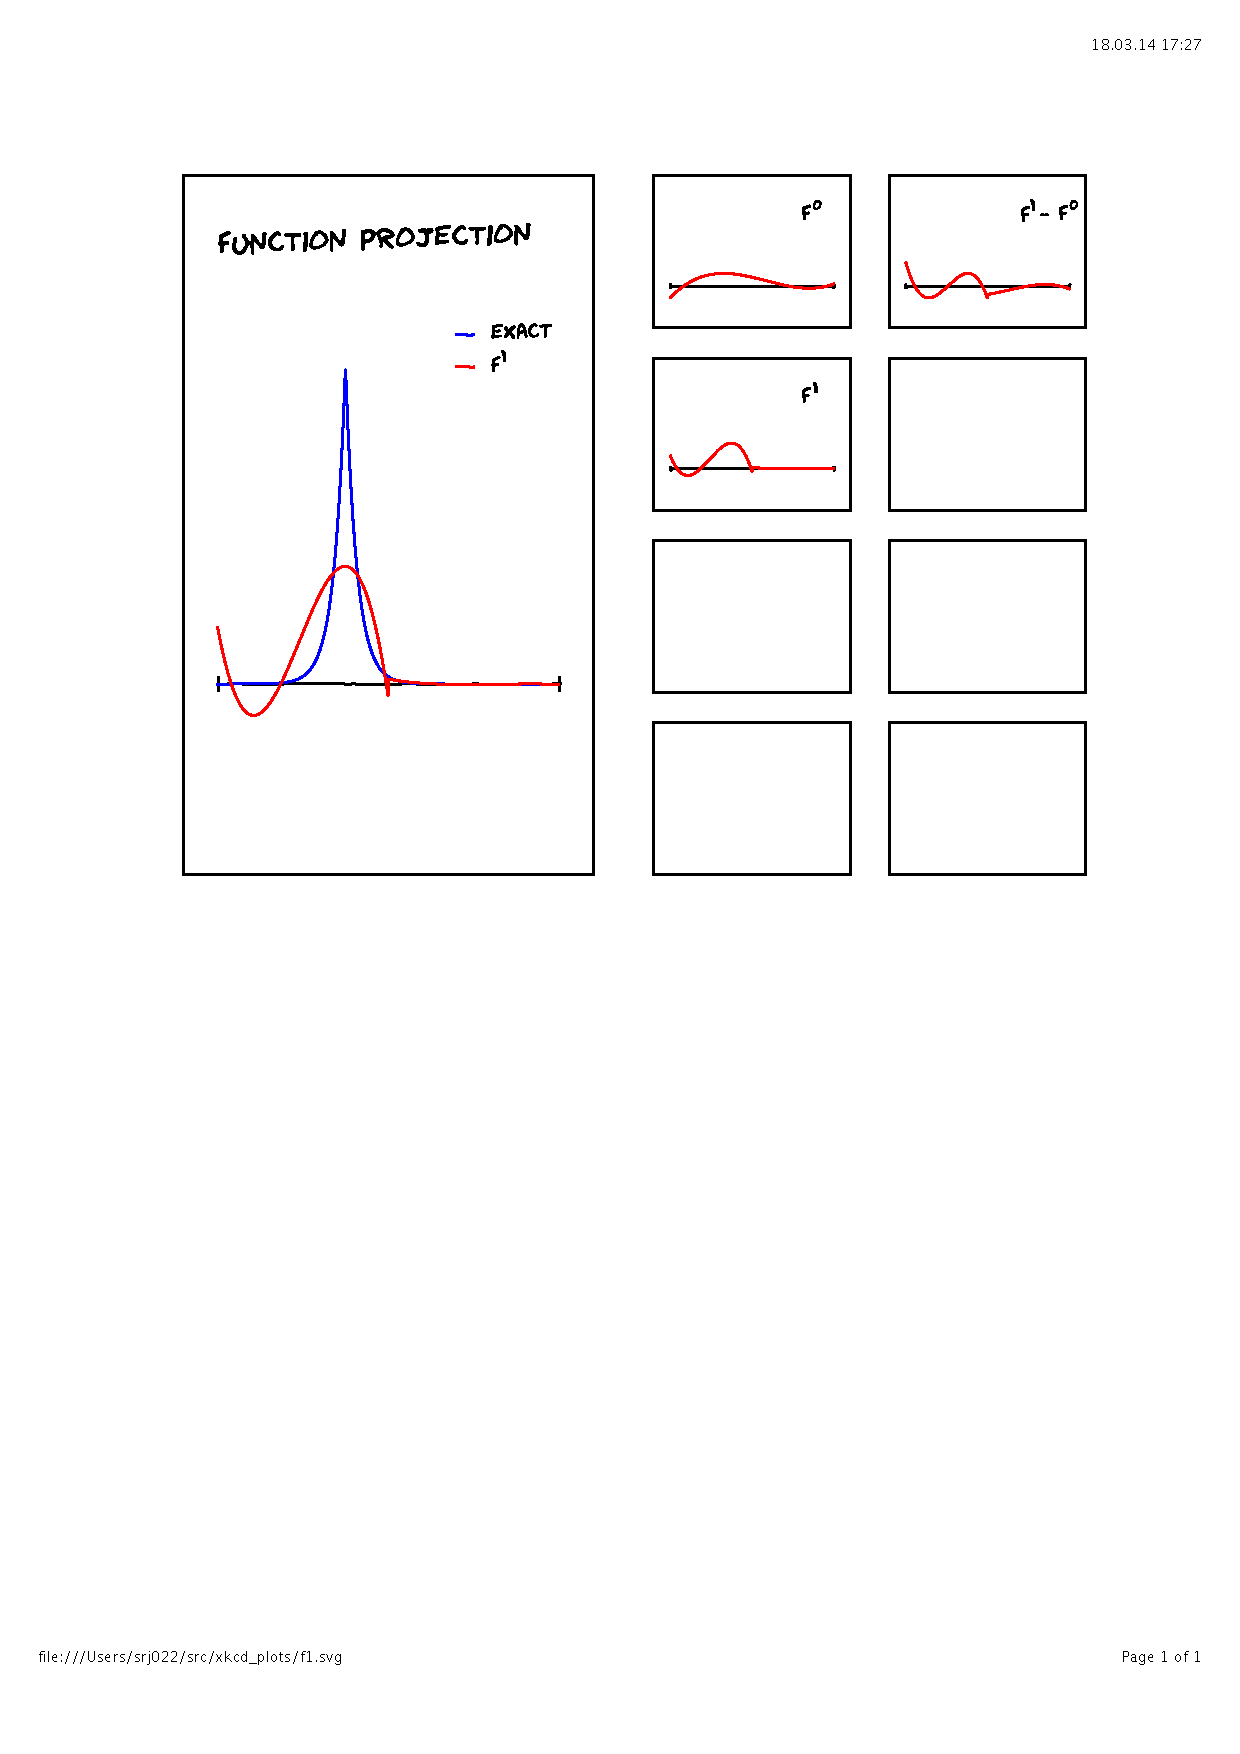
\includegraphics[clip, viewport=50 100 600 800, scale=0.5]
    {figures/f1.pdf}}
\only<3>{\ 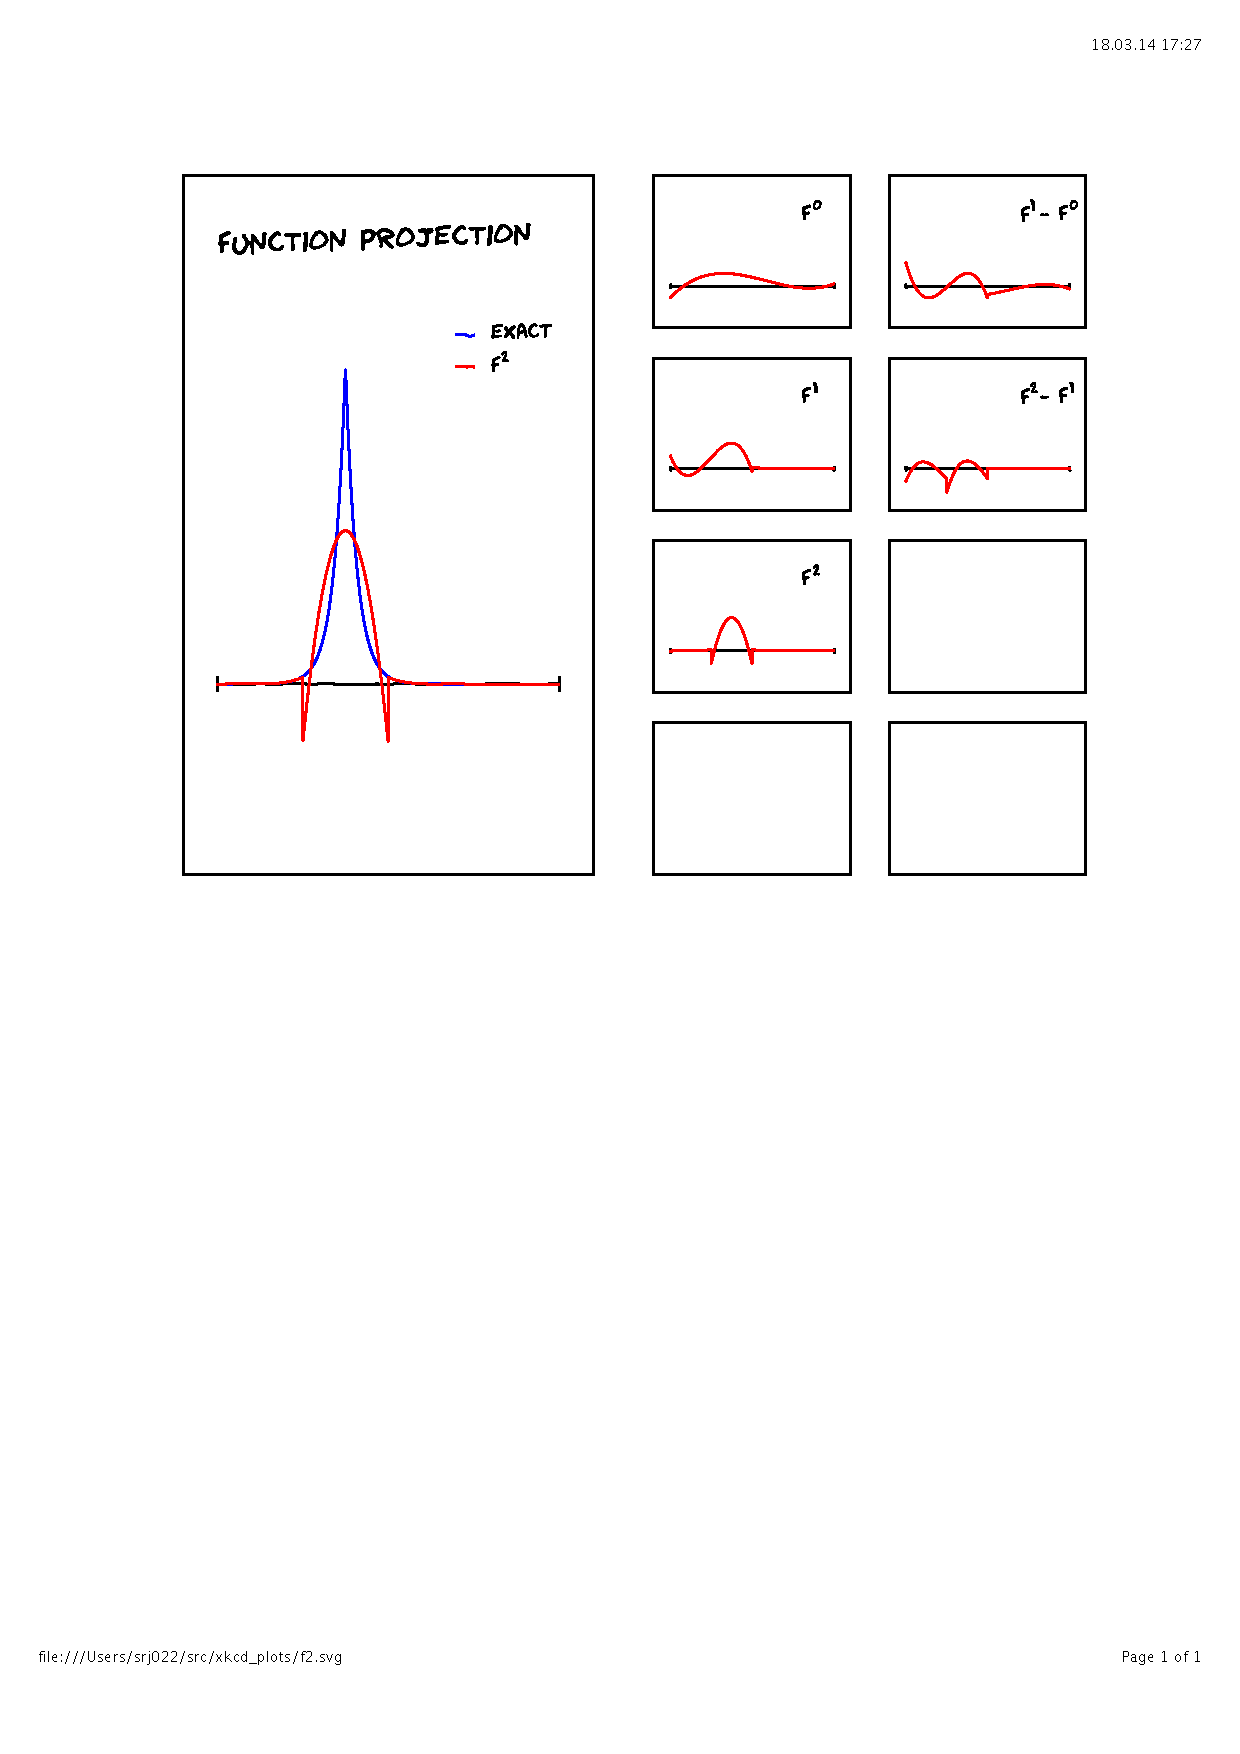
\includegraphics[clip, viewport=50 100 600 800, scale=0.5]
    {figures/f2.pdf}}
\only<4>{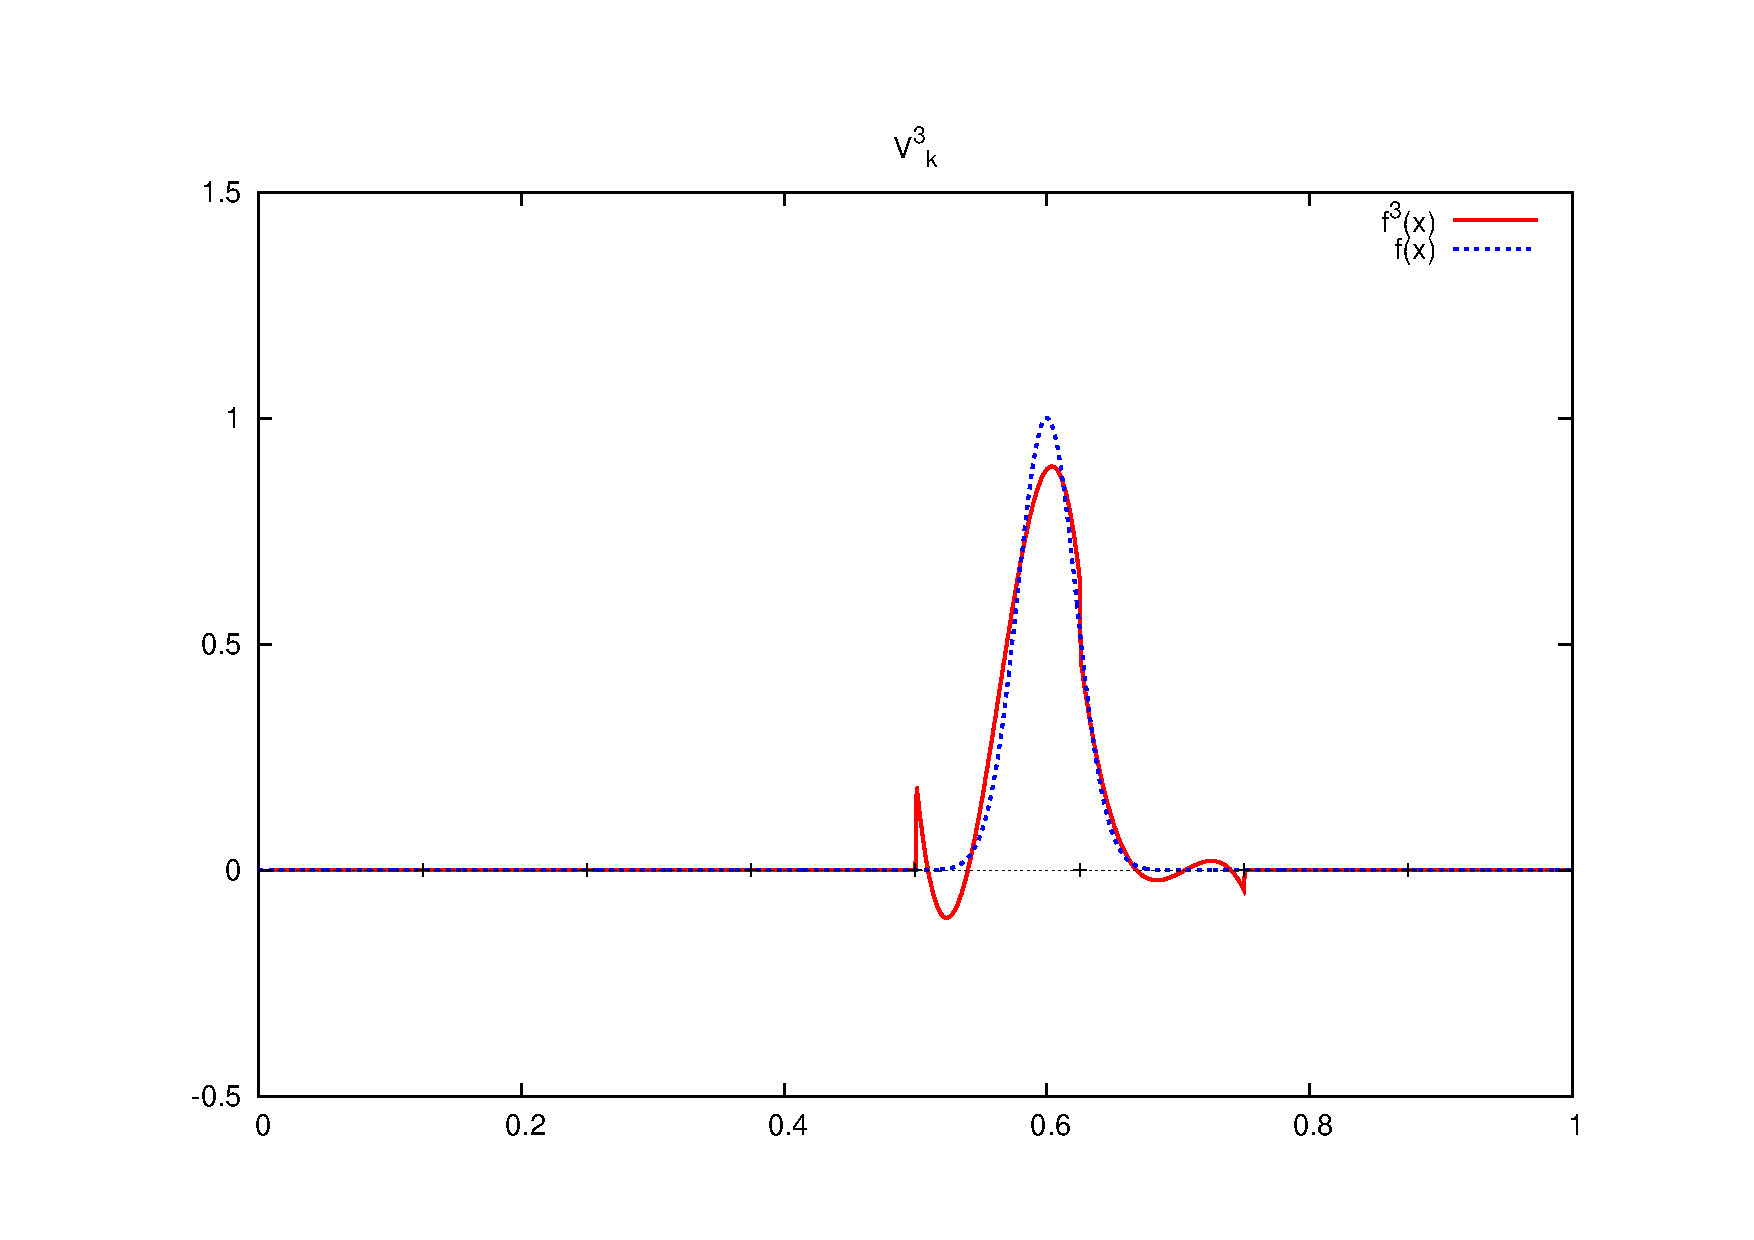
\includegraphics[clip, viewport=50 100 600 800, scale=0.5]
    {figures/f3.pdf}}
\only<5>{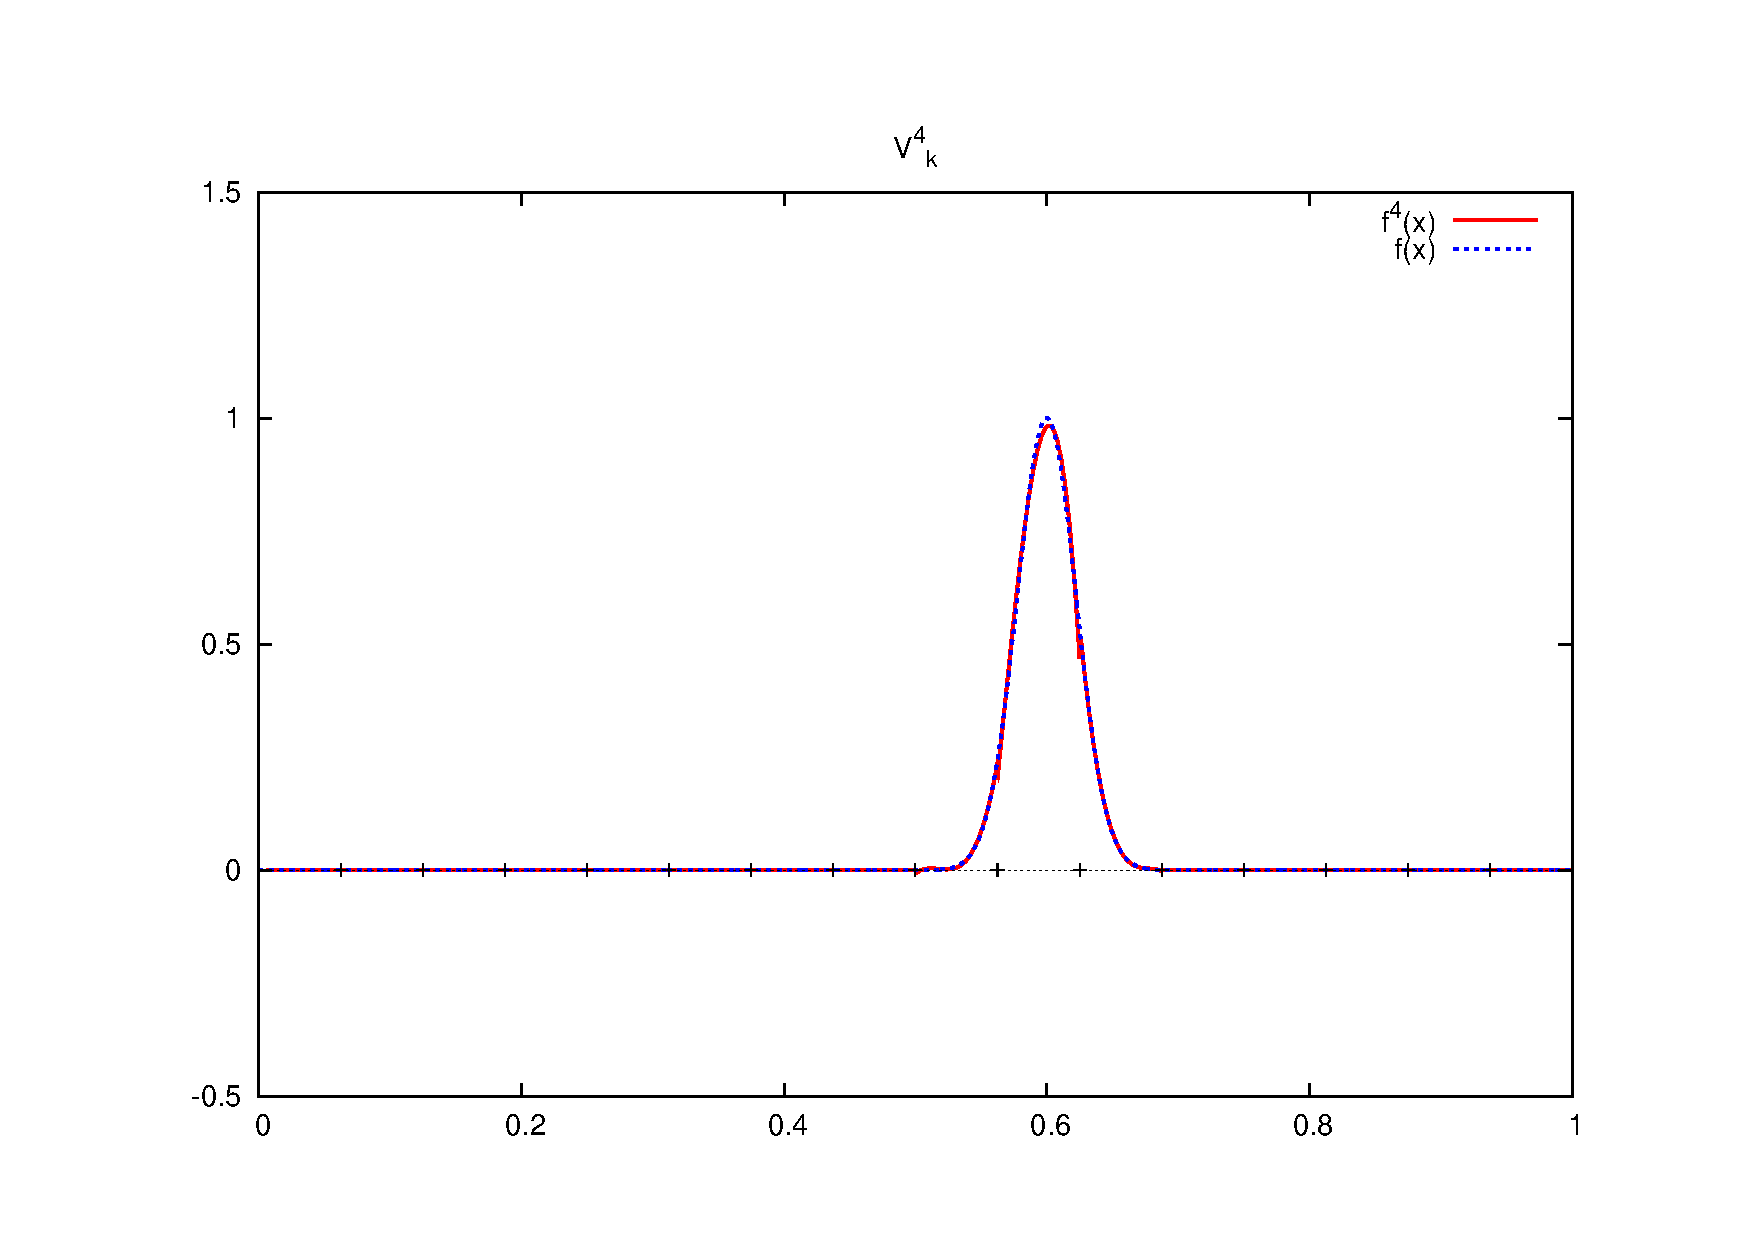
\includegraphics[clip, viewport=50 100 600 800, scale=0.5]
    {figures/f4.pdf}}
\end{frame}

%\begin{frame}
%\frametitle{Multiwavelets}
%\centering
%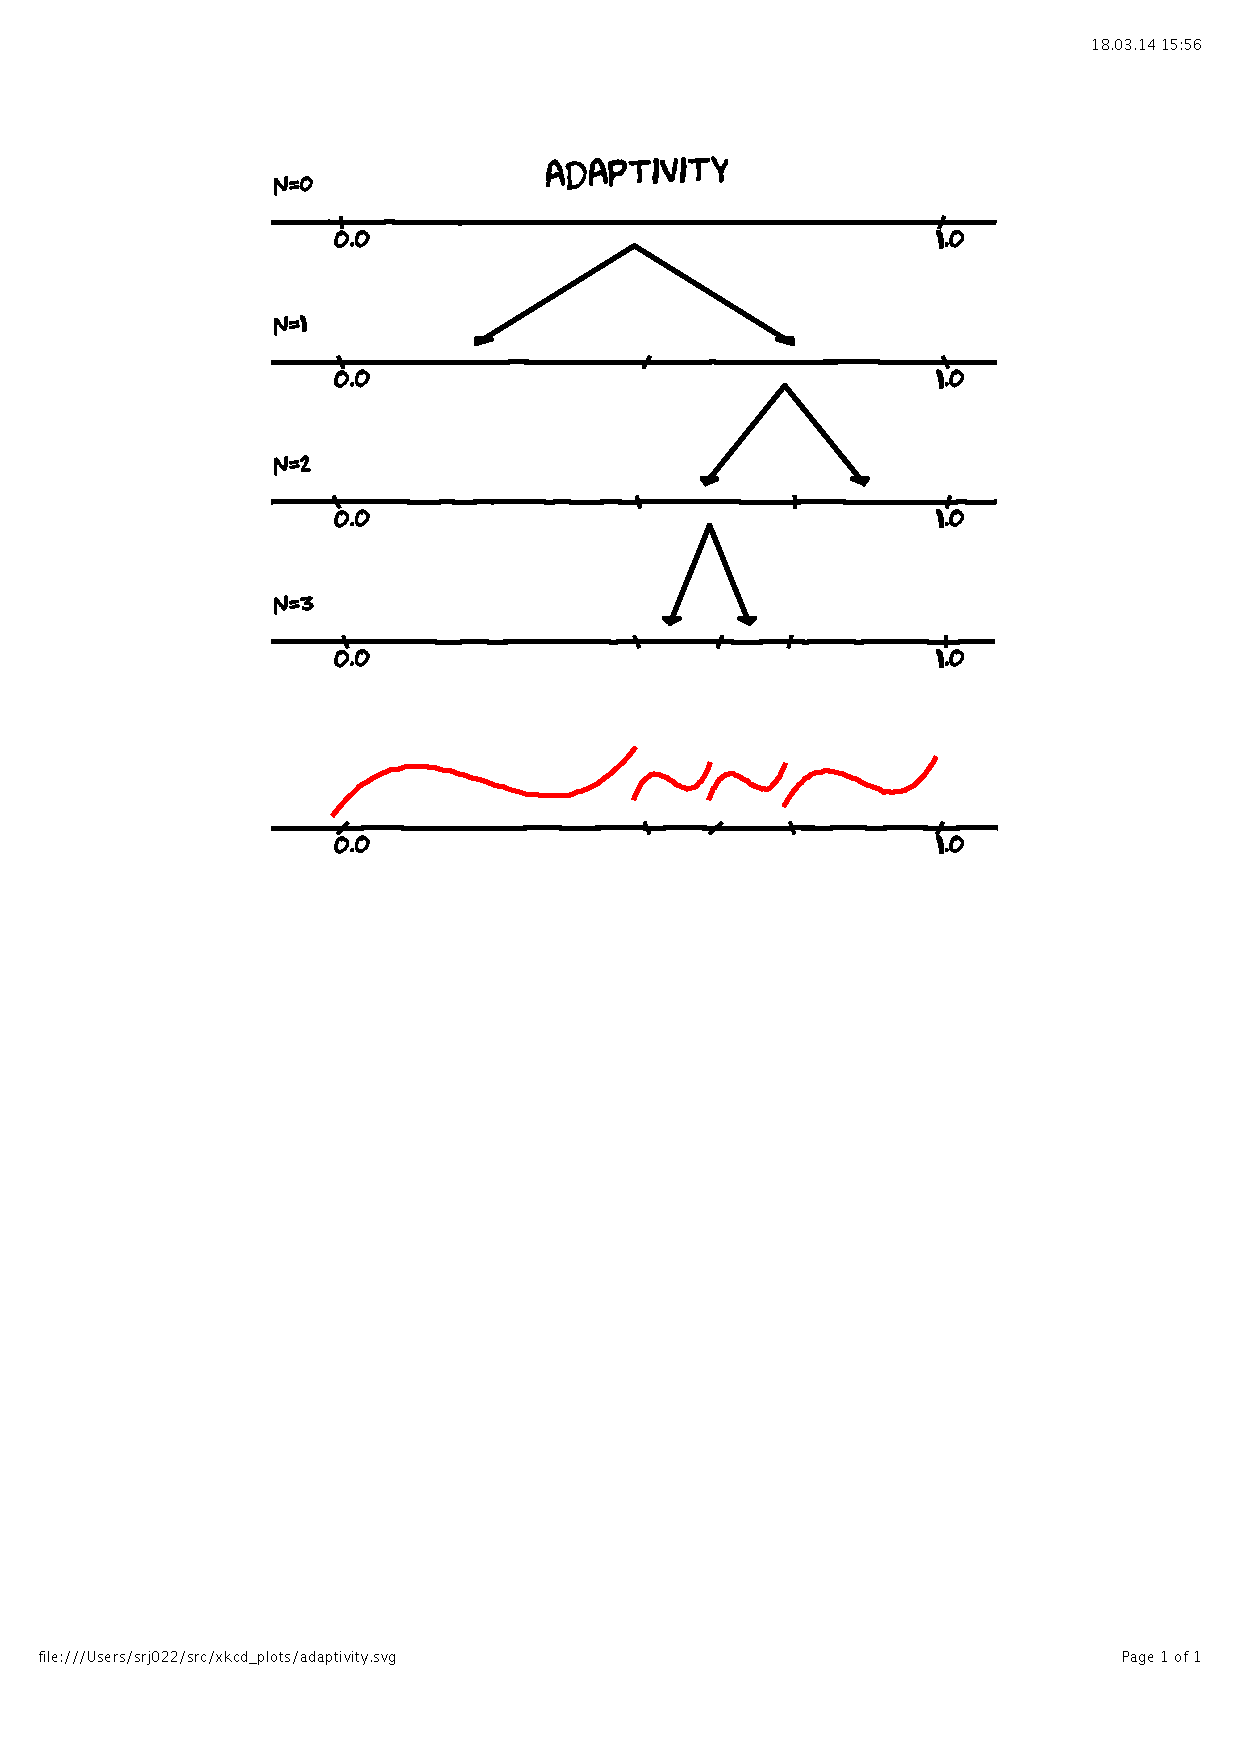
\includegraphics[scale=0.5, clip, viewport=100 400 500 800]{figures/adaptivity.pdf}
%\end{frame}

\begin{frame}
\frametitle{Multiwavelets}
\centering
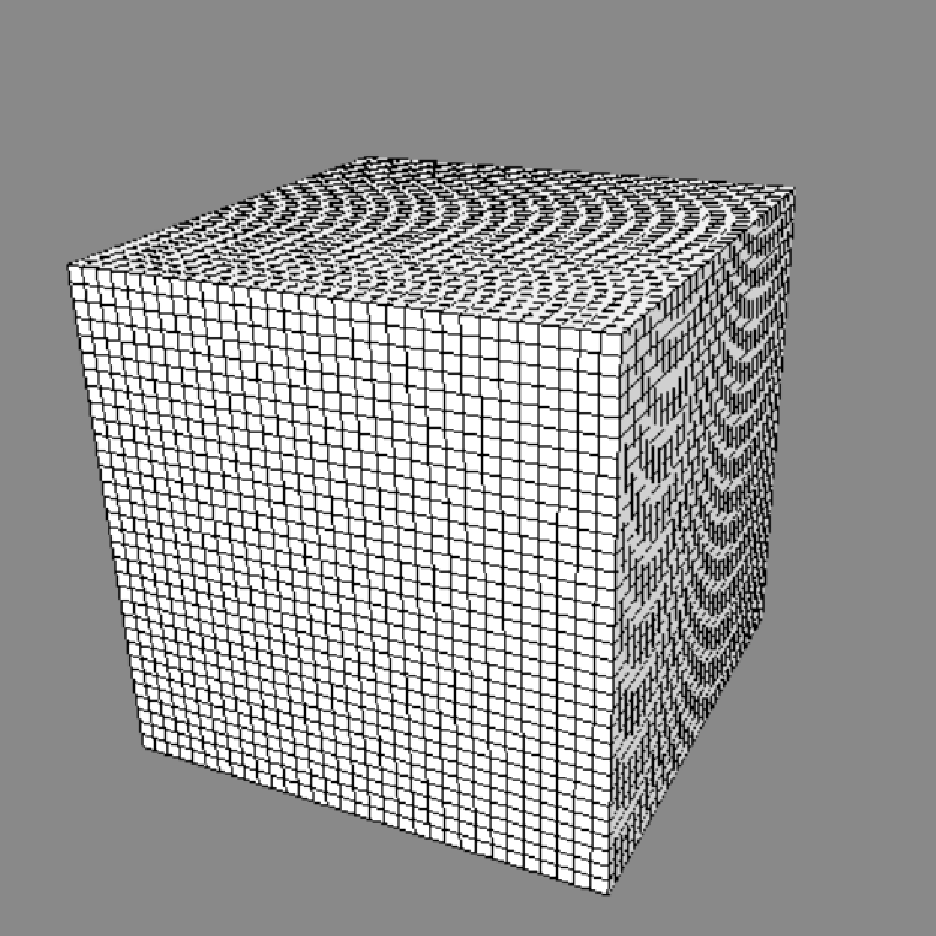
\includegraphics[scale=0.3]{figures/unifgrid.pdf}
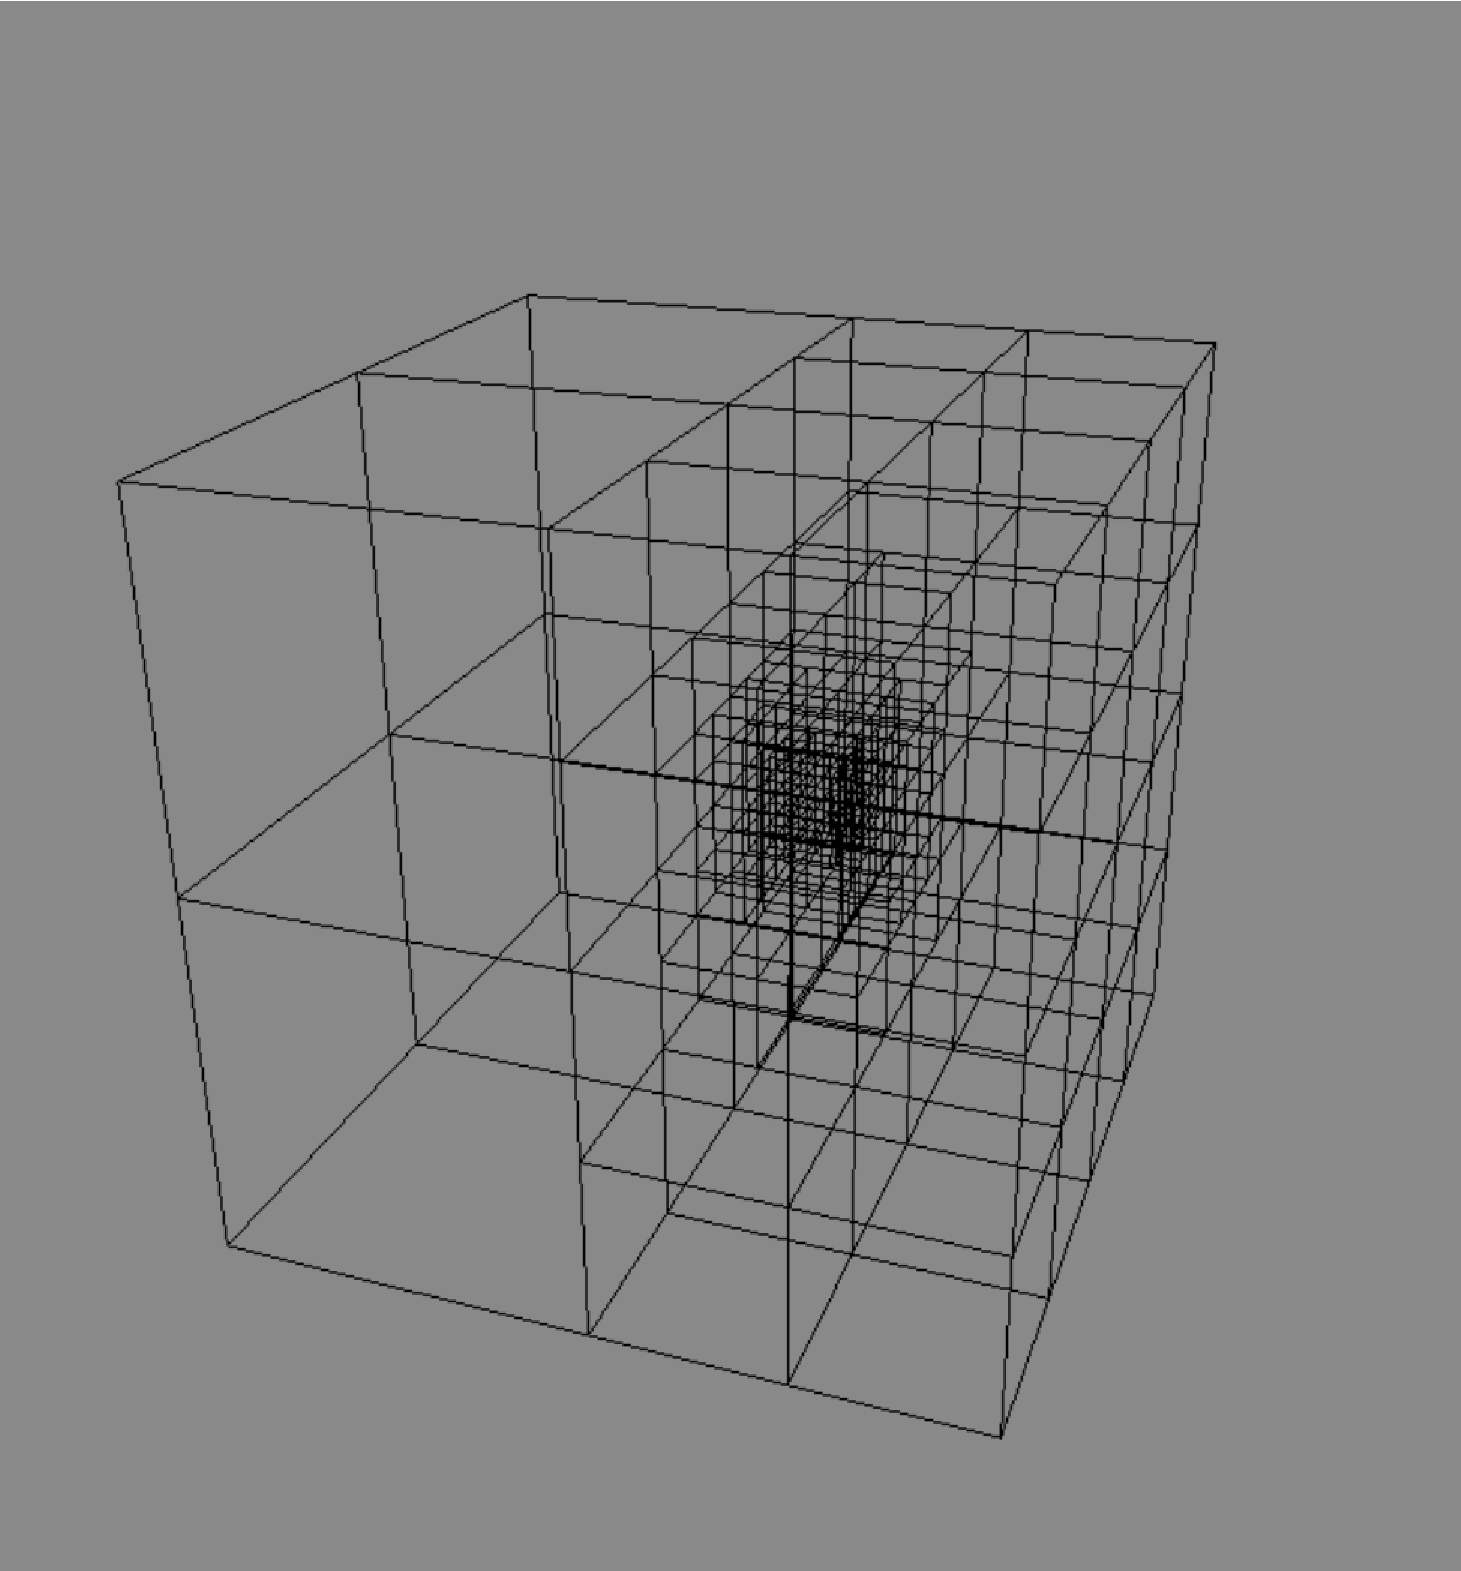
\includegraphics[scale=0.1788]{figures/adapgrid.pdf}
\end{frame}

%\begin{frame}
%\frametitle{Multiwavelets}
%\begin{columns}
%
%\begin{column}[b]{0.55\linewidth}
%\begin{itemize}
%    \item   \textbf{Wavelet functions} are piecewise polynomials
%    \item   \textbf{Wavelet projection} at scale $N$
%	\begin{equation}
%	    \nonumber
%	    df^n(x) = f^{n+1}(x) - f^{n}(x)
%	\end{equation}
%	\ \\
%    \item   Alternative \textbf{multiresolution} representation
%	\begin{equation}
%	    \nonumber
%	    f^N(x) = f^{0}(x) + \sum_{n=0}^{N-1} df^{n}(x)
%	\end{equation}
%    \item   Allows for \textbf{adaptive refinement} by local thresholding
%	\begin{equation}
%	    \nonumber
%	    \|df_l^n\| < \frac{\epsilon}{2^{n/2}}\|f\|
%	\end{equation}
%    \item   Representations with \textbf{guaranteed precision} $\epsilon$
%\end{itemize}
%\ \\
%\ \\
%\end{column}
%
%\begin{column}[b]{0.45\linewidth}
%\centering
%\includegraphics[scale=0.3, clip, viewport=100 400 500 800]
%    {figures/adaptivity.pdf}
%\end{column}
%
%\end{columns}
%\ \\
%\centering
%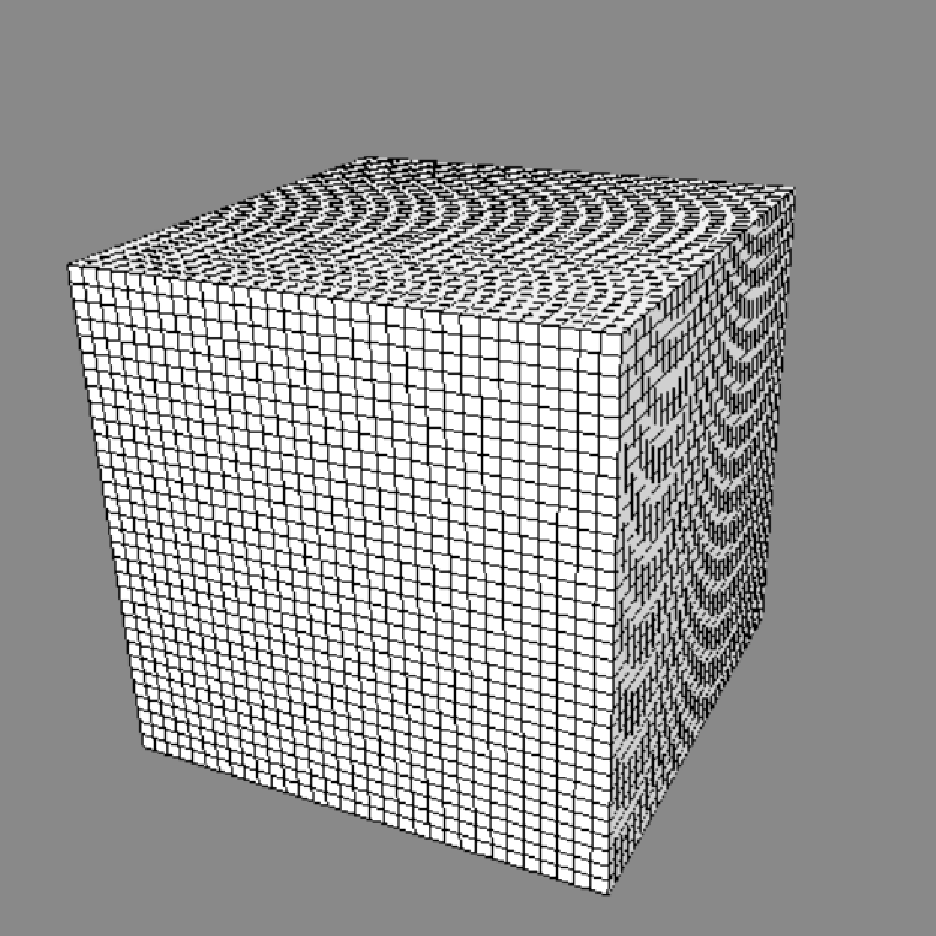
\includegraphics[scale=0.2]{figures/unifgrid.pdf}
%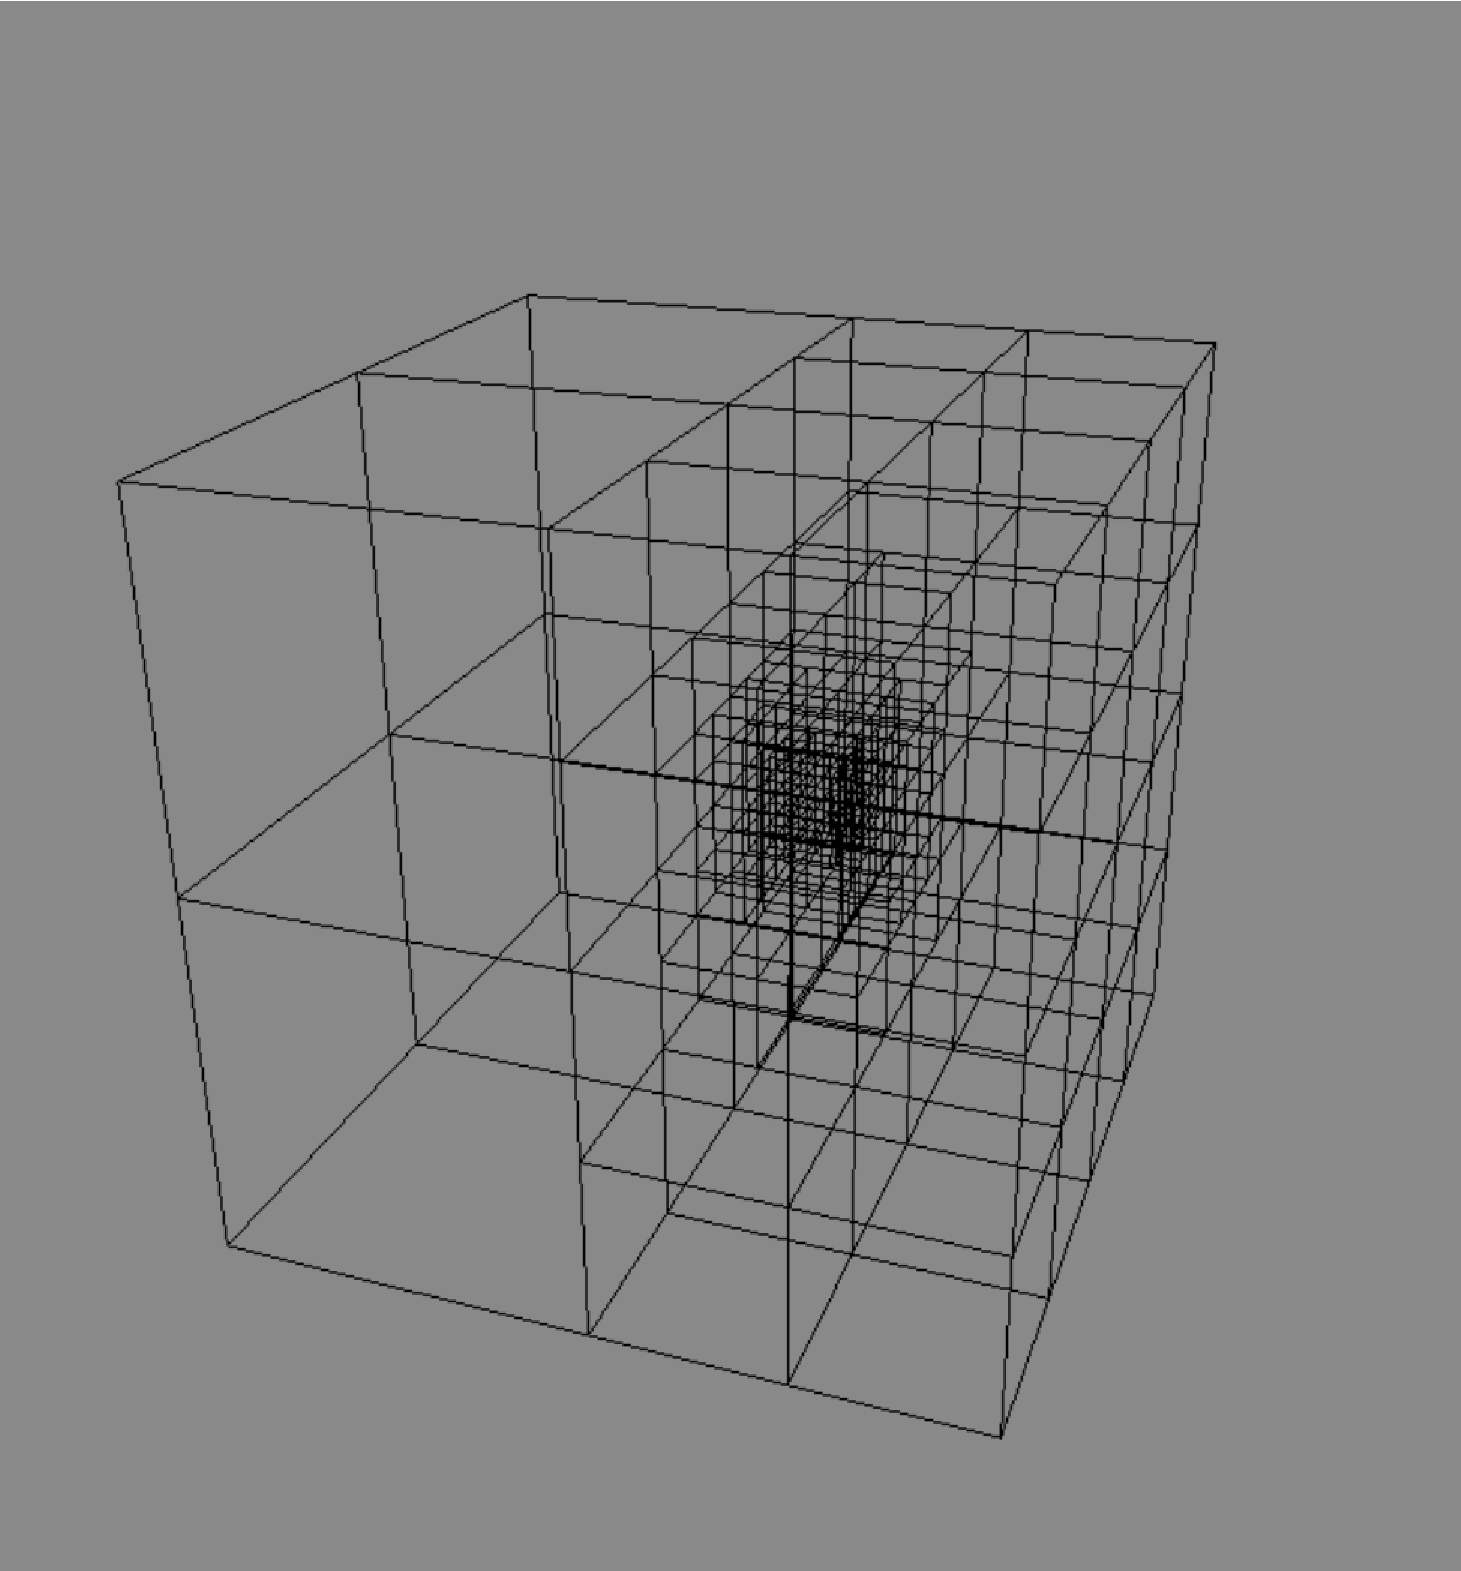
\includegraphics[scale=0.1192]{figures/adapgrid.pdf}
%\end{frame}


%\begin{frame}
%    \frametitle{Decreasing order polynomial basis}
%    \begin{columns}
%    \begin{column}[b]{0.7\linewidth}
%	\begin{itemize}
%	    \item   Multi-dimensional functions require many expansion coefficients\\
%		    \ \\
%	    \item   Try to reduce the memory footprint by varying the polynomial order\\
%		    \ \\
%	    \item   Specifically decreasing the order $k$ with increasing scale $n$
%	\end{itemize}
%	\ \\
%	\ \\
%	\ \\
%    \end{column}
%    \begin{column}[b]{0.3\linewidth}
%    \centering
%    \begin{figure}
%	\setlength{\unitlength}{.5mm}
%	\begin{picture}(93,46)
%	    \put( 0,10){\vector(1,0){60}} n- axis
%	    \put(61,10){$n$}
%	    \put(10,4){\vector(0,1){37}} k-axis
%	    \put(10,43){$k$}
%	    \put(40,38){$k(n)$}
%	    \put(-5,30){$k_{\max}$}
%	    \put(-5,15){$k_{\min}$}
%	    \put(25,5){$n_0$}
%	    \put(40,5){$n_1$}
%	    \put(10,30){\line(1,0){15}}
%	    \put(25,30){\line(1,-1){15}}
%	    \put(40,15){\line(1,0){15}}
%	    \multiput(40,10)(0,0.1){5}{\line(0,1){2}} 
%	    \multiput(25,10)(0,4){5}{\line(0,1){2}}
%	    \multiput(10,15)(6,0){5}{\line(1,0){2}}
%	\end{picture}
%    \end{figure}
%    \end{column}
%    \end{columns}
%    \ \\
%    \centering
%    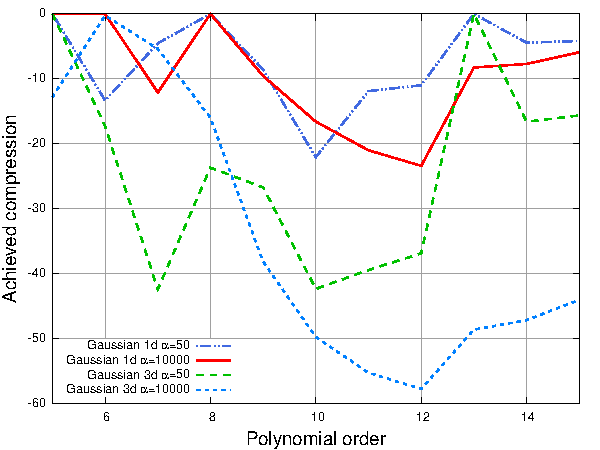
\includegraphics[scale=0.6]{figures/decrease.pdf}
%\end{frame}

